\section{Pillar 1: Language as Grounding Signal}%
\label{sec:pillar1}


In this pillar, we discuss the role of language in providing grounding for each component of the task in which an agent operates.As illustrated in Figure~\ref{fig:groundingsignal}, verbal feedback maps to specific MDP elements \citep{sutton1998reinforcement}: specifying what the agent should optimize (goals - \S\ref{sec:goal-grounding}), what it perceives (states- \S\ref{sec:state-grounding}), how it can act (actions- \S\ref{sec:action-grounding}), and what constitutes success (rewards- \S\ref{sec:reward-code}) \citep{ macglashan2017interactive}. This matters because many failures in language-based agents stem not from poor optimization but from poor grounding: feedback that cannot map to executable actions or valid reward conditions will not improve the agent. A common bottleneck across all four subcategories is the grounding gap. More detailed verbal specifications do not necessarily result in improved grounding. The critical factor is whether the mapping from language to MDP components is sufficiently precise for the agent to execute actions.
 
\begin{figure}[!t]
     \centering    
    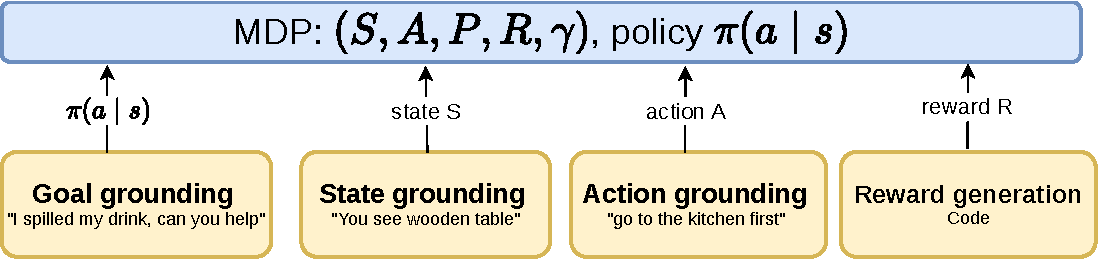
\includegraphics[width=1\linewidth]{paper_images/taxonomy3.pdf}
    
    \caption{\footnotesize Grounding of MDP components through natural language. Each subcategory maps verbal feedback to a specific element of the MDP: goal grounding specifies the objective, state grounding represents observations as text, action grounding resolves instructions to executable behavior, and reward code generation compiles language into executable reward functions.}
    \label{fig:groundingsignal}
\end{figure}

\subsection{Goal Grounding}%
\label{sec:goal-grounding}
Goal grounding uses verbal feedback to specify what the agent should achieve, requiring parsing instructions into objects, relations, and target conditions \citep{chaplot2018gated}, filtering plans by physical executability \citep{ahn2022can, driess2023palm}, and decomposing goals into verifiable subgoals. Recent work extends this to multi-agent coordination \citep{zhang2025towards}, hierarchical decomposition via offline RL \citep{hu2025divide}, and training from language specifications without manual reward functions \citep{li2026ground}. The open challenge is compositional generalization: agents must follow goals assembled from familiar primitives in unfamiliar combinations. BabyAI \citep{chevalier2018babyai} isolates this in gridworlds, and even state-of-the-art LLMs achieve only about 75\% coverage under compositional constraints \citep{sakai2025revisiting}, though compositional policy representations can improve sample efficiency on novel compositions \citep{cohen2025compositional}.



\subsection{State Grounding}%
\label{sec:state-grounding}
Where goal grounding defines what to achieve, state grounding defines what the agent perceives. Verbal state descriptions are most explicit in text-based environments \citep{yao2020keep, cote2018textworld}, but appear whenever visual or physical states are summarized into language. \citet{shridhar2020alfworld} show that agents trained on verbal state descriptions transfer to embodied 3D settings, demonstrating language as a modality-invariant state representation. Recent work includes closed-loop state feedback for robotic planning \citep{bhat2024grounding} and scene-graph-based grounding \citep{huang2025escacontextualizingembodiedagents}. A key challenge is information preservation, specifically whether the verbal abstraction retains sufficient signal for the policy to operate effectively.



\subsection{Action Grounding}%
\label{sec:action-grounding}
Given a goal and a perceived state, the agent must determine how to act. Action grounding resolves verbal instructions to specific skills, tool calls, or motor commands, requiring that instructions map to executable actions and that execution outcomes feedback as language to revise subsequent steps. \citet{huang2022inner} demonstrate this closed loop with Inner Monologue, while \citet{sharma2022correcting} show that short corrective utterances can amend mistaken steps without disrupting the rest of the plan. Recent systems have pushed toward tighter integration: multi-modal grounded replanning that corrects ambiguous instructions using visual cues \citep{kim2025multi}, constraint-aware visual programming for proactive failure detection \citep{zhou2025code}, corrective planning that handles physical, logical, and semantic errors across hierarchical control levels \citep{joublin2024copal}, and visually grounded task-and-motion planning that combines LLM reasoning with physical feasibility \citep{zhang2025llm}. The central challenge is granularity alignment: the same instruction can refer to a temporally extended skill (``make coffee''), a discrete subgoal (``go to the kitchen''), or a motor command (``close the gripper''), each demanding a different language-to-control interface.



\subsection{Reward Code Generation}%
\label{sec:reward-code}
The preceding subcategories ground objectives, observations, and actions in language. Reward code generation closes the loop by grounding success itself. This subcategory overlaps with Pillar~3 when generated rewards are used for training; we categorize it here because verbal feedback defines the reward function itself, becoming part of the MDP\added{, and Table~\ref{tab:hybrid} records the downstream training role explicitly. Under our inclusion criteria, the linguistic signal is consumed at specification time, so reward-code generation satisfies criterion (i) even though the compiled function later emits scalar rewards}. The distinguishing feature is compiling verbal descriptions into executable reward functions rather than using language as a direct learning signal. \citet{ma2024eureka} introduced Eureka, where an LLM generates and iteratively refines reward code based on training summaries, and \citet{xie2024text2reward} extended this to dense reward shaping. This area has seen rapid recent progress: CARD \citep{sun2025large} introduces dynamic trajectory-based feedback to refine reward code without per-iteration RL training, PROF \citep{sun2025prof} extends the paradigm to offline settings through preference optimization, and \citet{zeng2024video2reward} show that reward functions can be generated from video demonstrations. To ensure effectiveness, verbal feedback must be compilable, executable, and accurately reflect the original natural-language intent.
